\chapter{Probabilistic Programs}\label{chap:preliminaries}

This section formalises necessary ingredients and the~problem statement for probabilistic synthesis.
We will first introduce a~discrete-time Markov chain as the~simplest operation model for probabilistic programs.
Further,~we will describe a~Markov decision process representing a~similar model as a~Markov chain,~but it contains additional non-determinism.
These models play a~crucial role when synthesising probabilistic programs,~as we will see later in Chapter~\ref{chap:synthesis_methods}.
The~following definitions are inspired from the~existing sources,~mainly from~\cite{tacas21,Quatmann2016},~where a~more detailed description can also be found.

\section{Probabilistic Models}

% \MC{Navrhuju napsat nejakou uvodni vetu, ze MC je semantika prob programu a podobne trochu nize ze MDP nam dovoluji uvazovat o mnozine prog programu.}
We denote a~finite set of \textit{parameters} as $V$.
We consider \textit{parameters} over the~domain $\real$ ranged over by $x,y,z$ for the~following definitions.
Let $u: V \rightarrow \real$ denote a~\textit{valuation} for \textit{parameters} $V$.
We denote a~set of \textit{multi-affine multivariate polynomials} as $\mathbb{Q}_V$, where polynomial $f$ is defined over parameters $V$ and equal to $\sum_{i \leq M}{\prod_{v\in V_i}v \cdot a_i}$,~for appropriate $M \in \nat$, $a_i \in \rat$,~and $\forall \, 0 \leq i \leq m. \; V_i \subseteq V$.
We note that this set includes only the polynomials where the~variables have the~maximal degree equal to one,~i.e.,~$y^3 \notin \mathbb{Q}_V$, but $y \cdot z \in \mathbb{Q}_V$.
When we apply the~valuation $u$ to polynomial $f \in \mathbb{Q}_V$,~the~resulting instance yields a~real number $f[u] \in \real$,~in which all occurrences of variable $x \in f$ are replaced by $u(x)$.
We consider various types of (parametric) discrete probabilistic models.
We can look at them as the~transition systems with the~given state space where the~transitions are marked with polynomials in $\mathbb{Q}_V$~\cite{Quatmann2016}.

\begin{definition}[pMDP]
A parametric Markov decision process (pMDP) $\mathcal{M}$ is a tuple $(S, V, s_0, Act, \mathcal{P})$, where $S$ is a finite set of states, $V$ is a finite set of parameters over $\real$, $s_0 \in S$ is an initial state, $Act$ is a non-empty finite set of actions, and $\mathcal{P}: S \times Act  \times S \nrightarrow \mathbb{Q}_V$ is a transition function.
\end{definition}
\noindent
A~set $\mathit{Act(s) = \{ a \in Act \; \lvert \; \exists s' \in S. \mathcal{P}(s, a, s') \neq \; \perp \}}$ for state $s \in S$ represents the~\textit{available} actions.
The~model do not contains deadlock states,~since for each state $s \in S$ holds that the~action set $Act(s)$ is non-empty.
When holds $\lvert \mathit{Act(s)} \rvert = 1$ for each state $s \in S$,~such pMDP straightforward induces an~parametric Markov chain (pMC),~which has enabled only one action at each state.

\begin{figure*}[h!]
\centering
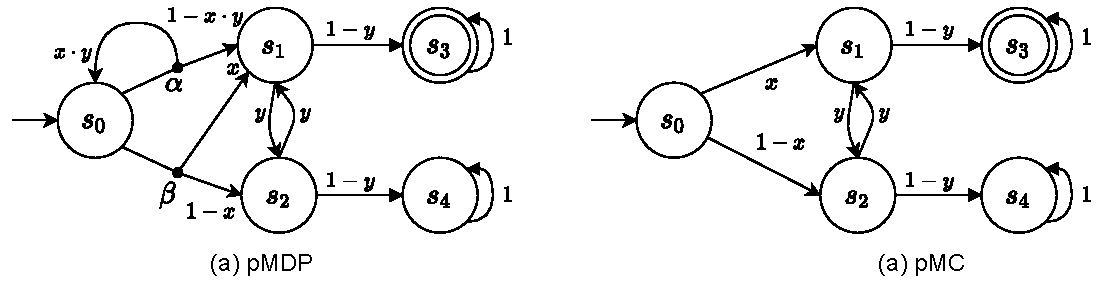
\includegraphics[width=1.0\textwidth]{figures/param_models.pdf}
\caption{The introduced kinds of parametric probabilistic models \,--\, pMDP and pMC.}%
\label{fig:param_models}%
\end{figure*}

\begin{example}[Parametric models]
We depict (a) pMDP and (b) pMC with parameters $\{x, y\}$ at Figure~\ref{fig:param_models}.
We mark an~initial state $s_0 \in S$  with an~arrow,~and the~target state $s_3 \in S$ with double lines.
We label the~transition from state $s \in S$ to $s' \in S$ by action $\alpha$ and corresponding $\mathcal{P}(s, \alpha, s')$,~if such transition is executable.
\end{example}

\begin{definition}[Distribution]
\cite{tacas21} 
    A \textit{discrete} distribution over a~finite or countably infinite set $X$ is a~function $\mu: X \rightarrow [0,1]$ s.t. $\sum_{x \in X} \mu(x) = \mu(X) = 1$.
    The~set of all distributions on $X$ is denoted $Distr(X)$.
    The support of a distribution $\mu$ is $supp(\mu) = \{ x \in X \, \lvert \; \mu(x) > 0 \}$.
    % A distribution is \textit{Dirac} if $\lvert supp(\mu) \rvert = 1$.
\end{definition}

\begin{example}[Parametric probabilistic models]
    Let $X = \{x_0, x_1, x_0\}$ be a finite set.
    Let function $\mu: X \rightarrow [0,1]$ defined as $\mu: [x_0 \mapsto \frac{1}{2}, x_1 \mapsto 0, x_2 \mapsto \frac{1}{2}]$ be a \textit{probability distribution} on $X$, i.e. $\mu \in Distr(X)$.
    The support of $\mu$ is $supp(\mu) = \{x_0, x_2 \}$, and for simplification, we writes such distributions as $\mu = \frac{1}{2} : x_0 + \frac{1}{2} : x_2$.
\end{example}


\begin{definition}[MDP]
    A pMDP $\mathcal{M}$ is Markov decision process (MDP) $M$ if $\mathcal{P}: S \times Act \times S \rightarrow Distr(S)$, so for each state $s \in S$ and each its action $\alpha \in Act(s)$ holds that $\sum_{s' \in S}{\mathcal{P}(s, \alpha, s')} = 1$.
\end{definition}
\noindent 
We can define in the same way a~MCs as the~special instance of pMCs.
We say,~that the~model is \textit{parameter-free} when for each its transition probability holds,~that it contains only constant values and not undefined parameters.
When we apply the~valuation $u$ to the~parametric model $\mathcal{M}$,~then we obtain the~instantiation of $\mathcal{M}$ at $u$ ($\mathcal{M}[u]$),~where each polynomial $f \in \mathcal{M}$ is replaced by $f[u]$.
We use the~valuation $u$ typically to substitute the~transition function $f$ by the~concrete probability $f[u]$.
When the~instantiated model $\mathcal{M}[u]$ yields an~MDP or MC,~we denote the~valuation $u$ as \textit{well-defined} since it returns the~probability distributions.

\begin{figure*}[h!]
\centering
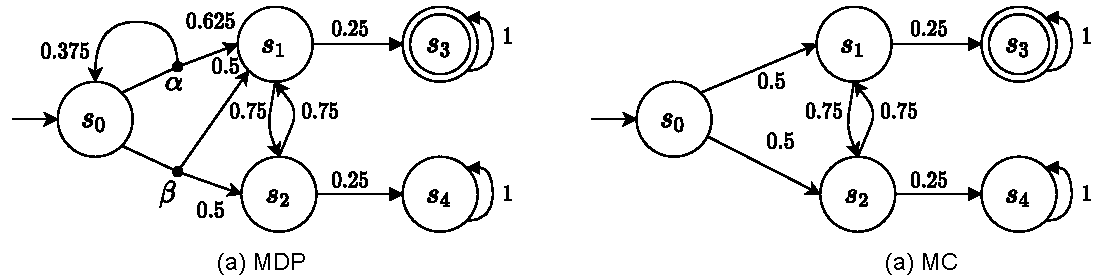
\includegraphics[width=1.0\textwidth]{figures/models.pdf}
\caption{The introduced kinds of probabilistic models \,--\, MDP and MC.}%
\label{fig:models}%
\end{figure*}

\begin{example}[Probabilistic models]
Figure~\ref{fig:param_models} depicts an pMDP and an pMC.
Let us consider the~following valuation $u: \{ x \mapsto 0.5, y \mapsto 0.75 \}$.
By applying this valuation to an~pMDP results in parameter-free MDP depicted at Figure~\ref{fig:models},~and the~same in the~case of MC instantiated from relevant pMC.
\end{example}

Instinctively,~we can imagine an~$MC$ as a~state-transition system with the~following semantics.
A~probability distribution for each state $\forall s \in S: \mathcal{P}(S)$ represents a~stochastic choice of firing the~transition from such state $s \in S$ to one of its successors states $s' \in supp(\mathcal{P(S)})$.
Consequently,~an~$MC$ defined with such semantics has a~\textit{Markov property} (memorylessness), which is essential when modelling systems and for efficient analysis.
This property declares that the~probability of the~transition from state $s \in S$ to state $s' \in supp(\mathcal{P(S)})$ depends only on the~current state,~and it is independent of the~taken path of chain to state $s$.
We can see that each state of an $MC$ disposes of a unique probability distribution over its possible successor states.
MDPs define an~extension of $MCs$ introducing a~non-deterministic choice between several probability distributions over each state.

A~(in)finite sequence $\pi = s_0 \overset{a_0}{\rightarrow} s_1 \overset{a_1}{\rightarrow} \dots$,~where $s_i \in S$,~$a_i \in Act(s_i)$,~and $\mathbb{P}(s_i, a_i)(s_{i+1}) \neq 0$ for all $i \in \mathbb{N}$ represents the~\textit{path} of an~MDP M.
For finite $\pi$, $last(\pi)$ denotes the last state of $\pi$,~and the~set of (in)finite paths of M we denotes as $Paths_{fin}^{M}\,(Paths^M)$.
When an~$MDP$ is currently in the~state $s \in S$,~it has a~non-deterministic choice of an action $a \in Act(s)$ leading to the~one possible probability distribution $\mathcal{P}(s)(a)$ over its successors' states.
These actions cause the~non-deterministic behaviour of an~$MDP$.
Still,~this property can be suppressed by applying a~\textit{scheduler},~which selects one specific action in each state,~i.e.,~transforms an~$MDP$ to an~$MC$.

% \begin{definition}[MDP]
% \cite{roman-DP}
%     A Markov decision process (MDP) $M$ is a~quadruple $\mdp$ ~where $S$ is a~finite set of states,~$s_0 \in S$ is an~initial state,~$Act$ is a~finite set of actions,~and $\mathcal{P}: S \times Act  \nrightarrow Distr(S)$ represents a~(partial) transition probability function. 
% \end{definition}

% A~set $\mathit{Act(s) = \{ a \in Act \; \lvert \; \mathcal{P}(s, a) \neq \; \perp \}}$ for state $s \in S$ represents the~\textit{available} actions.
% When holds $\lvert \mathit{Act(s)} \rvert = 1$ for each state $s \in S$,~such MDP straightforward induces an~MC.

\begin{definition}[Scheduler]
A scheduler for an pMDP $\mathcal{M} = (S, V, s_0, Act, \mathcal{P})$ is a function $\sigma: Paths_{fin}^{M} \rightarrow Act$ such that $\sigma(\pi) \in Act(last(\pi))$ for all $\pi \in Paths_{fin}^{M}$.
Scheduler $\sigma$ is memory-less if $last(\pi) = last(\pi') \Longrightarrow \sigma(\pi) = \sigma(\pi')$ for all $\pi, \pi' \in Paths_{fin}^{M}$.
The set of all schedulers of M is $\Sigma^M$.
\end{definition}
\noindent 
When we apply a~scheduler to an~pMDP,~then we obtain an~induced parametric Markov chain,~which does not contain any non-determinism.
In other words,~the~transition probabilities are obtained concerning the~choice of actions.

\begin{definition}[Induced pMC] \label{def:incuded_mc}
\cite{cegar}
An pMC induced by pMDP $\mathcal{M} = (S, V, s_0, Act, \mathcal{P})$ and $\sigma \in \Sigma^M$ is defined by $M_{\sigma} = ( Paths_{fin}^{M}, s_0, \mathbf{P}^{\sigma})$ where:
\begin{align*}
    \mathbf{P^{\sigma}}(\pi, \pi') = 
    \begin{cases}
        \mathcal{P}(last(\pi), \sigma(\pi))(s') \quad & if \; \pi' = \pi \overset{\sigma(\pi)}{\rightarrow} s' \\
         0 \quad & otherwise.
    \end{cases}
\end{align*}
\end{definition}


\section{Probabilistic Synthesis}
We use a~\textit{sketch}~\cite{sketching1,sygus}, ~which represents a~incomplete high-level description of a~probabilistic system,~to describe the~family of MCs.
It usually describes the~modelled system's fixed behaviour,~but it also contains the~undefined one represented by \textit{holes}.
They represent the~incomplete parts of a~program that must be instantiated so that the~final description satisfies a~given specification.
We note that the~holes correspond to parameters,~and their instantiation yields a~concrete Markov chain.
At follow, we formalise the sketch defining the set of designs:

\begin{definition}[Sketch]
Let $\sketch$ be a~sketch containing holes from the~set $\mathcal{H} = \left\{ H_k \right \}_k$ with $R_k$ being the~set of options available for hole $H_k$.
Let $\rlzf = \prod_k R_k$ denote the~set of all hole assignments (realizations),~$\sketch[r]$ denote the~program induced by a~substitution $r \in \rlzf$ and $\fmlr$ denote the underlying MC.
Note that the~set $\rlzf$ is exponential in $\lvert \mathcal{H} \rvert$.
\end{definition}
\noindent
We consider \textit{reachability} properties and \textit{expected reward} properties as specifications.

\begin{definition}[Specification]
In our work,~we focus on the~conjunctions of specifications with \textit{reachability} and \textit{expected rewards}.
Let $T$ be a~set of target states,~then the~reachability property $\varphi \equiv \reachability{\bowtie}{\lambda}{T}$ where $\bowtie \in \{<, \leq, >, \geq\}$ and $0 \leq \lambda \leq 1$ expresses that the~probability of reaching $T$ refers to $\lambda \in [0,1]$ in agreement with $\bowtie$.
Expected reward property $\phi \equiv \reward {\bowtie}{\lambda}{T}$ expresses that the~expected reward accumulated before $T$ is reached refers to $\lambda \in \mathbb{R}^+$ in accordance with $\bowtie \, \in \{<, \leq \}$.
Let $\mathcal{P}[r]$ be a~program induced by the~realisation $r$,~we denote $\mathcal{P}[r] \models \varphi$ when this program satisfies the~specification $\varphi$.
Let $\varPhi = \{ \varphi_i \}_{i \in I}$ be a~finite set of specifications,~when $\forall i \in I: \mathcal{P}[r] \models \varphi_i$ then we write $\mathcal{P}[r] \models \varPhi$.
\end{definition}

We aim to two kinds of synthesis tasks for a~given probabilistic program described with a~realisation set $\rlzf$,~and a~specification set $\varPhi$.
The first task tries to identify just one realisation $r \in \rlzf$ that satisfy the~given specification set $\varPhi$.
This task represents a~special instance of the~threshold synthesis,~which tries to divide the~realisation set $\rlzf$ into two subsets based on their satisfiability.
We do not address this synthesis task in our work.
The second task on which we focus our attention is finding a~realisation that minimises or maximises a~given objective.

\begin{definition}[Feasibility]
Find a realisation $r \in \rlzf$ such that $\mathcal{P}[r] \models \varPhi$. 
\end{definition}

\begin{definition}[Minimality] \label{def:minimality}
For property $\phi_{\min}$, find a realisation $r^* \in \rlzf$ such that:
$$r^* \in \argmin_{r \in \rlzf} \left \{ \prob[\sketch[r] \models \phi_{\max}] \mid \sketch[r] \models \varPhi \right \}.$$.
\end{definition}

We defined only minimal synthesis task for probability property,~but its variants for maximisation and expected rewards may be defined analogously.
Moreover, we focus also to a relaxed variant of minimal synthesis, the so-called \textit{$\varepsilon$-minimal synthesis}, defined as follows: $\mathcal{P}[r^*] \models \varPhi \; and \; 
\mathbb{P}[\mathcal{P}[r^*] \models \varphi_{min}] \leq (1 - \varepsilon) \cdot \min_{r \in \mathcal{\overline{R}}} \{ \mathbb{P}[\mathcal{P}[r] \models \varphi_{min}] \; \lvert \; \mathcal{P}[r] \models \varPhi \}.$

\begin{example} (Synthesis problem)
Assume an~MCs family $\fml$ from Example~\ref{exam:mcfamily} and the~specification $\phi = \reachability{\geq}{0.1}{\{s_1\}}$.
The solution to the~feasibility synthesis problem is,~for example,~the~realisation $r_0$, since $\mathcal{D}_{r_0}$ has a~probability of $\frac{2}{3}$ to reach state $s_1$.
For $\varPhi = [F \; \{s1\}]$,~the~solution to the~maximal synthesis problem on MCs family $\fml$ is the~realisation $r_2$,~as MC $\mathcal{D}_{r_2}$ has a~probability equal to one to reach state $s_1$.
\end{example}

\section{Region Model Checking}
We consider valuation sets that mapping parameter to the~value within a~specified interval. 
We introduce a~technique for approximate checking pMC instances concerning the~valuation in such a~set.
Firstly,~we introduce definitions for \textit{regions} and the~considered task of model checking.
Subsequently,~we define the~construction of \textit{over-approximation},~which will be subsequently \textit{reduce} to an~MDP problem.
The~definitions in this section are inspired mainly by~\cite{Quatmann2016}.

\subsection{Regions}
\begin{definition}[Region]
Let $V = \{ v_1, v_2, \dots, v_n \}$ be a~set of parameters and $\forall \, v_i \in V. \; \mathcal{B}(v_i) = \{b_1, b_2 \}$ rational bounds for each parameter $v_i$.
These parameter bounds induce for parameter $v_i$ its interval $I(v_i) = [b1, b2]$ where holds $b1 \leq b2$.
Let $U = \{ u \; \lvert \; \forall \, v_i \in V. \; u(v_i) \in I(v_i) \}$ be a~set of valuations, which we call a region for parameters set $V$.
\end{definition}
\noindent
Note that regions represent instances $\mathcal{M}[u]$ derived from the~parametric model $\mathcal{M}$.
As we presented above,~these model instances are \textit{well-defined} when they hold some assumptions,~so we shift them also to regions.

\begin{definition}[Well-defined region]
Let $\mathcal{M}$ be a~parametric probabilistic model.
Let $r$ be a~region for set of parameters $V$,~we call the~region $v$ \textit{well-defined} for $\mathcal{M}$,~when holds for each \textit{polynomial} $f \in \mathcal{M}$ either $f[u] > 0$ or  $f$ can be reduced to 0 $f = 0$,~and for each \textit{valuation} $u \in r$ holds that $u$ is \textit{well-defined} for model $\mathcal{M}$.
\end{definition}
\noindent
The~first condition guarantees that both models $\mathcal{M}$ and $\mathcal{M}[u]$ have the~same topology,~and the~second one says that $\mathcal{M}[u]$ represents a~probabilistic model (MDP or MC).

\begin{figure*}[h!]
\centering
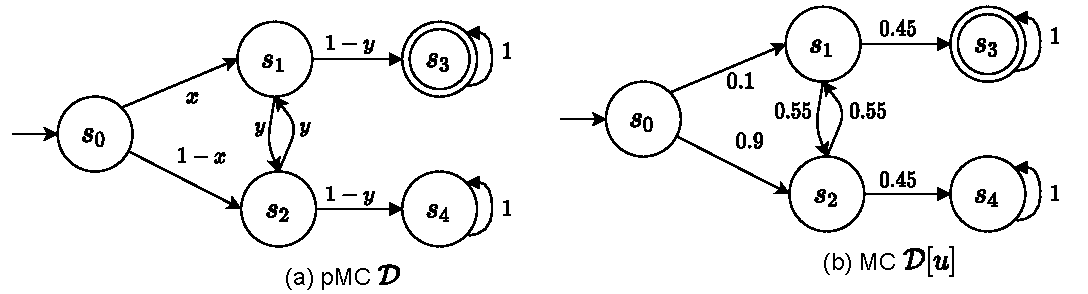
\includegraphics[width=1.0\textwidth]{figures/param_instance.pdf}
\caption{A \textit{parametric} MC $\mathcal{D}$, and instantiated MC $\mathcal{D}[u]$ from it.}%
\label{fig:param_instance}%
\end{figure*}

\begin{example}[Region]
Let us consider the pMC $\mathcal{D}$ depicted at Figure~\ref{fig:param_instance},~the~region $r$ defined as $r = [0.1, 0.5] \times [0.5, 0.6]$ and valuation derived from it $u = (0.1, 0.55)$.
Applying a~valuation $u$ to parametric model $\mathcal{D}$,~yields a~parameter-free MC $\mathcal{D}[u]$ depicted at Figure~\ref{fig:param_instance}(b).
Note,~that this instantiated model $\mathcal{D}[u]$ has the~same topology as the~original pMC.
We can say that the~considered region $r$ is \textit{well-defined},~since this holds for each possible valuation $u' \in R$,~respectively for an~instance $\mathcal{D}[u']$ derived from it.
At the~contrary,~the~region $r' = [0.0, 0.5] \times [0.75, 1.0]$ is not \textit{well-defined},~because for example the~valuation $v' = (0.0, 1.0)$ yields an~MC which has no transition from $s_0$ to $s_1$,~or from $s_1$ to $s_3$,~so it has different topology as original pMC $\mathcal{D}$.
\end{example}

We will introduce a~\textit{satisfaction relation} for regions,~which defines whether the~given region $r$ and parametric model $\mathcal{M}$ satisfies the~specification $\varphi$.
We denote $\mathcal{M}, r \models \varphi$ when each instance derived from the parametric model $\mathcal{M}$ described with a region $r$ satisfies the analysed specification $\varphi$.

\begin{definition}[Region satisfaction relation]
The relation $\models$ for a~well-defined region $r$,~a~parametric model $\mathcal{M}$,~and a~given specification $\varphi$ is defined as follows:
\begin{align*}
    \mathcal{M}, r \models \varphi \Longleftrightarrow \forall u \in r. \; \mathcal{M}[u] \models \varphi
\end{align*}
\end{definition}
\noindent
When holds $\mathcal{M}, r \not\models \varphi$,~then this statement implies $\exists u \in r. \; \mathcal{M}[u] \not\models \varphi$.
On the contrary,~when holds $\mathcal{M}, r \models \neg\varphi$ which implies $\forall u \in r. \; \mathcal{M}[u] \not\models \varphi$,~this is different from the~first case.
Let $\mathcal{D} = (S, V, s_0, \mathcal{P})$ be an pMC, $r$ a~well-defined region for this pMC $\mathcal{D}$,~and $\varphi = \reachability{\geq}{\lambda}{T}$ a~given reachability property.
When we want to conclude whether the~region $r$ is \textit{live} or not,~we need to compute for each valuation $u \in r$ the~corresponding (\textit{minimal} or \textit{maximal}) reachability probability.
We define the following equivalences to detect whether given \textit{region} $r$ is \textit{live} or not:
\begin{align*}
    \mathcal{D}, r \models \varphi \Longleftrightarrow (\argmin_{u \in r} \prob[\mathcal{D}[u] \models F \; T]) \geq \lambda \\
    \mathcal{D}, r \models \neg\varphi \Longleftrightarrow (\argmax_{u \in r} \prob[\mathcal{D}[u] \models F \; T]) < \lambda \\
\end{align*}
Since the corresponding probability $\prob[\mathcal{D}[u], r \models F \; T]$ can be represented as a rational function $f$, and the region $r$ is well-defined, there exists the valuation inducing the minimal or maximal reachability probability on considered region $r$.

\begin{example}[Region model checking]
Let $\mathcal{D}$ be an~MC depicted at Figure~\ref{fig:param_instance}(a),~and we  consider a~region $r = [0.1, 0.5] \times [0.5, 0.6]$.
Let us suppose,~that we want to obtain a~valuation $u \in r$ maximising $\prob[\mathcal{D}[u], r \models F \; \{s_3 \}]$,~so the~probability that from an~initial state $s_0$ will be reached the state $s_3$.
Let us observe,~that the~single state from which the~state $s_3$ is not reachable is the~state $s_4$,~which is reachable only from state $s_2$.
Therefore,~to achieve the~highest probability will be the~best strategy minimising the~probability to reach state $s_2$.
We can conclude,~that the~parameter $x$ should has its value $u(x)$ as high as possible,~i.e.,~$u(x)= 0.5$.
Now,~we consider the~state $s_1$,~when we want to reach state $s_3$ from it,~then the~parameter $y$ should has its value $u(x)$ as low as possible.
However,~at the~same time we would need the~highest possible value for the~parameter $y$ to reach state $s_1$ from state $s_2$.
An~exhaustive analysis is required to find an~optimal value for parameter $y$, due to this trade-off.
\end{example}

\subsection{Substitution of pMCs}
We will introduce a~technique based on the~dropping of parameters dependencies in the~different states.
Thanks to the removal of these dependencies,~we can then effectively compute an~\textit{optimal} solution.
In order to compute minimal (or maximal) probability we have to make a discrete choice over valuations $\mathit{v}: V \rightarrow \real$ with $\mathit{v}(v_i) \in \mathcal{B}(v_i)$.
The~key idea consists of doing such a~choice locally at each state,~which allow us to construct the~\textit{parameter-free MDP} out of the~pMC $\mathcal{D}$ and the~region $r$.
The non-deterministic choices in this constructed MDP represent each valuation which is required to consider.

\begin{definition}[Substitution-pMC] \label{def:sub_mc}
Let $\mathcal{D}_{sub}^{r} = (S, s_0, Act_{sub}, \mathcal{P}_{sub})$ be an MDP representing the parameter-substitution of a pMC $\mathcal{D} = (S, V, s_0), \mathcal{P})$ and a region $r$, where holds $Act_{sub} = \biguplus_{s \in S}\{ \mathit{v}: V_s \rightarrow \real \; \lvert \; \mathit{v}(v_i) \in \mathcal{B}(v_i) \}$ and
\begin{align*}
    \mathcal{P}_{sub}(s, \mathit{v}, s') = 
    \begin{cases}
        \mathcal{P}(s, s')[\mathit{v}] \quad & if \; v \in Act_s \\
        0 \quad & otherwise.
    \end{cases}
\end{align*}
\end{definition}
\noindent
Intuitively,~the parameter-substitution $\mathcal{D}_{sub}^r$ of a~pMC $\mathcal{D}$ and a~region $r$ chooses an~action $\mathit{v}$ in state $s$ which corresponds to the~assigning of extremal values $\mathcal{B}(v_i)$ to the~parameter $v_i$. 
Note that the~non-deterministic choices introduced by this substitution depend only on the~values $\mathcal{B}(v_i)$ of the parameter $v_i$ in the~region $r$.

\begin{example}[Substitution-pMC]
Let us consider pMC $\mathcal{D}$ depicted at Figure~\ref{fig:param_instance}(a) and also the~introduced region $r = [0.1, 0.5] \times [0.5, 0.6]$ as above.
Figure~\ref{fig:sub_mc}(a) depicts the~\textit{substitution} of MC $\mathcal{D}$,~which includes non-deterministic choices instead of outgoing transition from states $s_0, s_1, s_2$ in the~original pMC $\mathcal{D}$.
In more precise,~we choose the~\textit{upper} or \textit{lower} bound for the~corresponding interval of the~parameter in each state.
The~green lines depict the~transitions that belong to the~action for the~lower bound,~and red lines for the~upper bound.
We note,~that states $s_3$ and $s_4$ contains only constant outgoing transition and therefore they have not any choices.
Figure~\ref{fig:sub_mc} depicts an~MC $(\mathcal{D}_{sub_r})^\sigma$ which is induced by the~scheduler $\sigma$ on MDP $\mathcal{D}_{sub_r}$.
\end{example}

\begin{figure*}[h!]
\centering
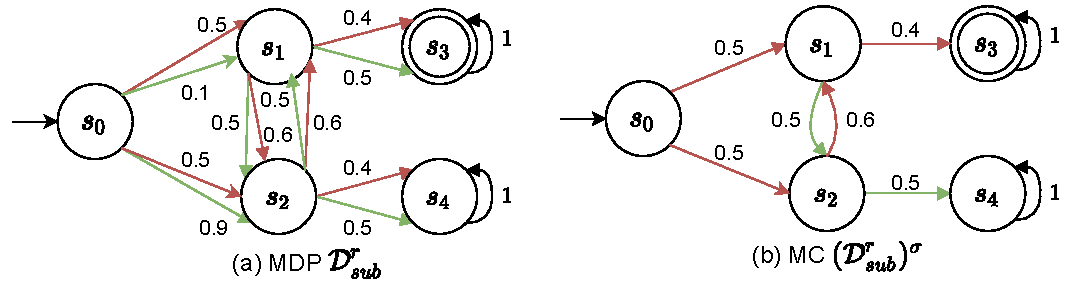
\includegraphics[width=1.0\textwidth]{figures/sub_mc.pdf}
\caption{A \textit{parameter-substitution} MDP $\mathcal{D}_{sub_r}$, and instantiated MC $(\mathcal{D}_{sub_r})^\sigma$.}%
\label{fig:sub_mc}%
\end{figure*}
\noindent
According to Theorem 1 which was defined and proved in~\cite{Quatmann2016}, we list the following:

\begin{theorem}[]
Let $\mathcal{D} = (S, V, s_0, \mathcal{P})$ be an~pMC,~$r$ a~region defined over this pMC $\mathcal{D}$,~and $T \subseteq S$ a~set of target states of $\mathcal{D}$,~then holds:
\begin{align*}
    \argmin_{u \in r} \prob[\mathcal{D}[u] \models F \; T] \geq \argmin_{\sigma \in \Sigma^{\mathcal{D}_{sub}^{r}}} \prob[(\mathcal{D}_{sub}^{r})^\sigma \models F \; T] \\
    \argmax_{u \in r} \prob[\mathcal{D}[u] \models F \; T] \leq \argmax_{\sigma \in \Sigma^{\mathcal{D}_{sub}^{r}}} \prob[(\mathcal{D}_{sub}^{r})^\sigma \models F \; T]
\end{align*}
\end{theorem}
\noindent
We define the following consequence straightforward from this statement:
\begin{theorem} \label{def:sub_mc_check}
Let $\mathcal{D} = (S, V, s_0, \mathcal{P})$ be an pMC,~$r$ a~well-defined region defined over this pMC $\mathcal{D}$,~then holds:
\begin{align*}
    \mathcal{D}_{sub}^{r} \models \reachability{\leq}{\lambda}{T} \Longrightarrow \mathcal{D}, r \models & \; \reachability{\leq}{\lambda}{T} \\
    \mathcal{D}_{sub}^{r} \models \reachability{>}{\lambda}{T} \Longrightarrow \mathcal{D}, r \models & \; \neg\reachability{\leq}{\lambda}{T}
\end{align*}
\end{theorem}
\noindent
Therefore,~we can use the~standard approaches for MDP model checking to check whether $\mathcal{D}, r \models \varphi$,~by applying these techniques to model $\mathcal{D}_{sub}^r$.
When the model checking of this considered over-approximation yield an~inconclusive results,~we refine the~regions to sub-regions and repeat the~control.

\subsection{Substitution of pMDPs}
In the~previous section,~we introduced a~technique to apply the~standard MDP model checking to the~parametric MCs. 
This technique substitutes outgoing transitions with non-deterministic choices representing the~relevant bounds of the~parameter related to this transition.
Now,~we generalise this technique to parametric MDPs,~or in general,~systems that include non-determinism.
In addition to the~choices over actions that the~MDP implicitly contains,~this technique also adds options over valuations concerning the~considered parameters.
This added level of non-determinism leads to a~game with two players.
The~first player represents the~original MDP non-determinism,~and the~second player the~abstracted parameters,~which results in a~stochastic game.

\begin{example}[MDP Substitution]
Let $\mathcal{M} = (S, V, s_0, Act, \mathcal{P})$ be an~pMDP depicted at Figure~\ref{fig:sub_mdp}(a).
Note that an~initial state $s_0$ can choice from two actions $\alpha$ and $\beta$.
When we consider the~scheduler $\sigma = \{ s \mapsto \beta \}$,~then by applying it to pMDP $\mathcal{M}$ we obtain pMC,~which we can subsequently transform to parameter-substitution MC,~as depicted at Figure~\ref{fig:sub_mdp}(b).
The~parameter substitution of a~MDP $\mathcal{M}$ returns an~SG $\mathcal{G}$ which is depicted at Figure~\ref{fig:sub_mdp}(d).
\end{example}

\begin{figure*}[h!]
\centering
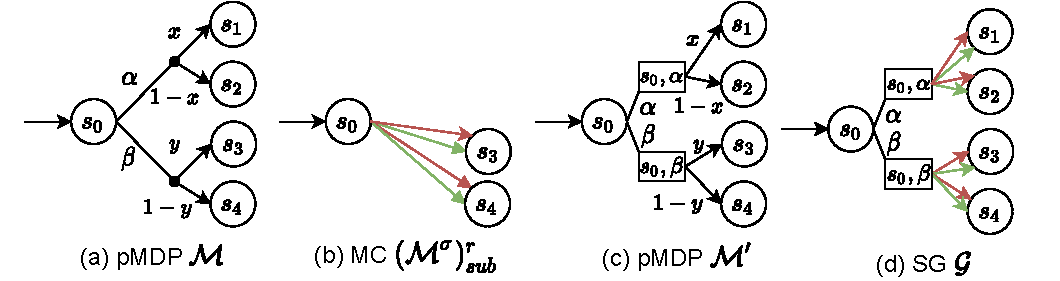
\includegraphics[width=1.0\textwidth]{figures/mdp_sub.pdf}
\caption{Illustration of the substitution of a pMDP.}%
\label{fig:sub_mdp}%
\end{figure*}
\noindent
When constructing the~\textit{parameter substitution} of a~pMDP,~we first need to construct its substitution,~which separates probabilistic choices from non-deterministic actions.
In the~first step,~we split each state $s \in S$ into set $\{s \} \; \uplus \; \{ (s, \alpha) \; \lvert \; \alpha \in Act(s) \}$,~and then we add a~transition with the~probability of $1$ from state $s$ to state $(s, \alpha)$ and move the~probabilistic choice concerning action $\alpha$ from $s$ to $(s, \alpha)$.
After applying of these operations,~we obtain a~pMDP $\mathcal{M}'$,~depicted in Figure~\ref{fig:sub_mdp}(c).
We can see that this MDP has clear non-deterministic choices leading to the~newly added states of the~form $(s, \alpha)$,~which on the~contrary,~have clear probabilistic choices.
As we said above,~by introducing parameter substitution on the~probabilistic states,~we obtain the~stochastic game $\mathcal{G}$,~depicted in Figure~\ref{fig:sub_mdp}(d).
The~first player represents the~original pMDP non-determinism,~while the~second one decides whether the~lower or upper bounds of the~parameters will be set.

\begin{definition}[Substitution-pMDP]
Let $\mathcal{M} = (S, V, s_0, Act, \mathcal{P})$ be an~pMDP,~and $r$ well-defined region.
A~\textit{stochastic game} $\mathcal{M}_{sub}^r = (S_{\circ} \uplus S_{\square}, s_0, Act_{sub}, \mathcal{P}_{sub})$ is the parameter-substitution of $\mathcal{M}$ over $r$ if $S_{\circ} = S$, $S_{\square} = \{ (s, \alpha) \; \lvert \; \alpha \in Act(s) \}$, $Act_{sub} = Act \uplus (\biguplus_{(s, \alpha) \in S_{\square}}Act_s^\alpha)$ where $Act_s^\alpha = \{\mathit{v}: V_s^\alpha \rightarrow \real \; \lvert \; \mathit{v}(v_i) \in \mathcal{B}(v_i) \}$, and
\begin{align*}
    \mathcal{P}_{sub}(t, \beta, t') = 
    \begin{cases}
        1 \quad & if \; t \in S_\circ \; and \; t' = (t, \beta) \in S_\square, \\
        \mathcal{P}(s, \alpha, t')[\beta] \quad & if \; t = (s, \alpha) \in s_\square, \beta \in Act_s^\alpha, and \; t' \in S_\circ, \\
        0 \quad & otherwise.
    \end{cases}
\end{align*}
\end{definition}
\noindent
The~constructed stochastic game $\mathcal{G} = \mathcal{M}_{sub}^r$ induced by various schedulers for the~first player $\circ$ relates with the~substitution in the~pMCs induced by schedulers from $\mathcal{M}$. 
In more precise,~the~schedulers $\sigma \in \Sigma^M_\circ$ for the~first player $\circ$ coincide with the~schedulers in $\mathcal{M}$.
Therefore,~the~models $\mathcal{G}^\sigma$ and ($\mathcal{M}^\sigma)_{sub}^r$ induced by the~scheduler $\sigma$ induce the~same reachability probabilities.
Thus,~we can substitute $\mathcal{M}$ directly and preserve the~reachability probability,~instead of performing the~substitution on the~pMC induced by $\mathcal{M}$ and $\sigma$.

\begin{theorem}
Let $\mathcal{M} = (S, V, s_0, Act, \mathcal{P})$ be an pMDP,~$r$ a~well-defined region defined over this pMC $\mathcal{D}$,~then holds:
\begin{align*}
    \mathcal{M}_{sub}^{r} \models_{\emptyset} \reachability{\leq}{\lambda}{T} \Longrightarrow \mathcal{M}, r \models & \; \reachability{\leq}{\lambda}{T} \\
    \mathcal{M}_{sub}^{r} \models_{\circ} \reachability{>}{\lambda}{T} \Longrightarrow \mathcal{M}, r \models & \; \neg\reachability{\leq}{\lambda}{T}.
\end{align*}
\end{theorem}
\noindent
Therefore,~similar as in the~introduced pMC case,~we can determine whether $\mathcal{M}_{sub}^r \models \varphi$ by analysing a~stochastic game.
For more details about proofs of listed definitions and theorems please refer to~\cite{Quatmann2016}.



\section{Families of Markov Chains}
This thesis considers a~parametric transition probability function as an~explicit representation of an~MCs family.
Such explicit representation relieves the~presentation and provides to describe exciting and practical problems for probabilistic synthesis.
On the~other hand,~arbitrary probabilistic programs permit the~modelling of more complex and independent parameter structures~\cite{cegar}.
In this thesis and our implementation,~we consider a~more flexible high-level modelling language,~see Section~\ref{sec:pris_language}.

We want to focus on families of (parametric) Markov chains having different topologies of the~state space and having undefined transition probabilities.
Such families have different sets of reachable states and also different probabilities of reaching individual states.
More specifically,~we consider the~family,~which is parametrised by a~finite set of discrete parameters $K$ and a~finite set of parameters $V$ over the~domain $\real$.

\begin{definition}[Family of pMCs]
\cite{cegar}
    A~\emph{family of pMCs} $\fml$ is a~quintuple $\family$  where $S$ is a~finite set of \emph{states}, $\sinit \in S$ is an~\emph{initial state},~$K$ is a~finite set of parameters with domains $T_k \subseteq S$ for each $k \in K$, $V$ is a finite set of parameters over the domain $\real$,~and $\fpm : S \times K \nrightarrow \mathbb{Q}_V$ is a~family of parametric transition probability functions.
\end{definition}

The~transition probability function $\fpm$ of pMCs family $\fml$ maps each state $s \in S$ to the~probability distribution over parameters from $K$, where the transitions are labelled with polynomials in $\mathbb{Q}_V$.
As we mentioned above,~these parameters from both sets $K$ and $V$ represent undefined system specifications when the~probabilistic synthesis is considered.
This function $\fpm$ yields a~specific pMC when we instantiate each parameter $k \in K$ with the~specific value from its domain $T_k \subseteq S$.
We call such instantiated pMC as \textit{realisation},~and the~following definition describes it.

\begin{definition}[Realisation]
\cite{cegar}
A~\emph{realization} of a~family $\fml = \family$ of pMCs is a~function $r: K \rightarrow S$ s.t.~$\forall k \in K :  r(k) \in T_k$. 
A~realization~$r$ yields a pMC $\mathcal{D}_r = (S, V, \sinit,\fpm(r))$,~where $\fpm(r): S \times K \nrightarrow \mathbb{Q}_V$ represents the~parametric transition probability matrix where each parameter $k \in K$ is substituted with $r(k)$. 
Let $\rlzf$ denote the~set of all (parametric) realisations for $\fml$.
\end{definition}

A~set $\prod_{k \in K} T_k$ representing all possible parameter combinations values has the~same semantics as a~set $\rlzf$ representing all family realisations with different topology of the~state space.
In other words,~we can define the~\textit{size of the~family} of pMCs in the~following way: $\lvert \fml \rvert := \lvert \prod_{k \in K} T_k \rvert = \lvert \rlzf \rvert = \prod_{k \in K} \lvert T_k \rvert$.
The~family size $\lvert \fml \rvert$ is finite because of the~finiteness of each parameter domain $T_k \subseteq S$,~but it is exponential in the~number of parameters $\lvert K \rvert$.
The~individual pMCs within the~family share the~same state space $S$,~but their set of reachable states can vary.
We emphasise that,~from the point of view of program synthesis,~such defined size of the~family does not indicate the~maximum number of realisations that must be examined.
This size indicates the~number of parametric realisations with different topologies,~which,~however, may still be inconclusive due to continuous parametric regions.
We note $\rlz$ as the~sub-families induced from the~whole family $\rlzf$.

\begin{example}[Family of MCs]\label{exam:mcfamily}
Let $\fml = \family$ be a~family of pMCs,~where $S = \{s_0, s_1, s_2, s_3\}$,~$K = \{ k_0, k_1, k_2, k_3 \}$ with domains $T_{k_0} = T_{k_1} = \{s_1, s_2\}$,~$T_{k_2} = \{ s_0 \}$,~and $T_{k_3} = \{ s_3 \}$,~and $V = \{ x, y \}$.
The parametric transition function $\fpm$ is defined as follows:
\begin{align*}
    \fpm(s_0) &= x : k_0 + (1-x) : k_1  \\
    \fpm(s_1)  &= y : k_2  + (1-y) : k_3 \\
    \fpm(s_2) &= 1.0 : k_0  \\
    \fpm(s_3)  &= 1.0 : k_3
\end{align*}
Figure~\ref{fig:mcfamily} draws the~pMCs family $\fml$ that correspond to all possible realisations: $\lvert T_{k_0} \rvert \cdot \lvert T_{k_1} \rvert = 2 \cdot 2 = 4$.
We note that these pMCs have a~different topology of the~underlying state space,~resulting in different sets of reachable states.
\end{example}

\begin{figure}[ht!]
\centering
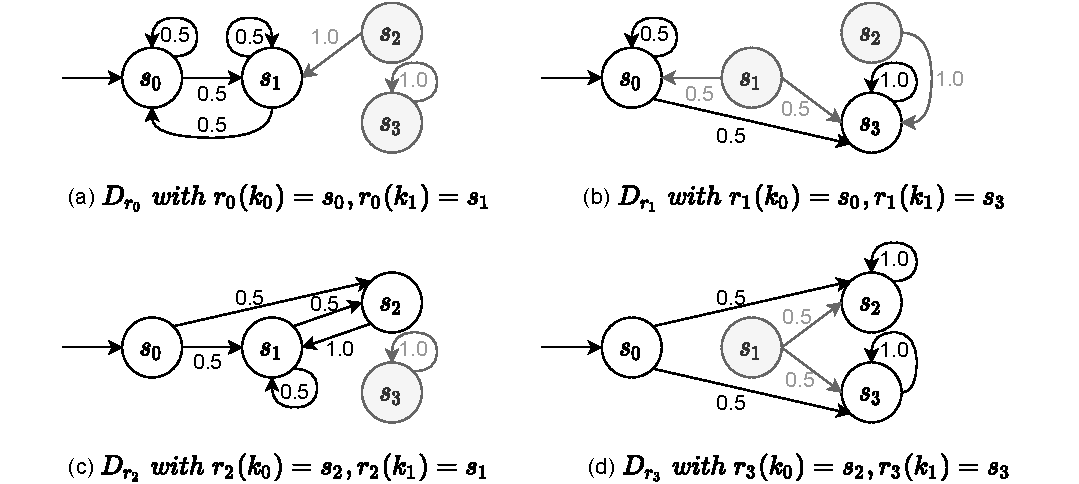
\includegraphics[width=0.9\textwidth]{figures/MCFamily.pdf}
\caption{A family $\fml$ of four various realisations. Unreachable states are greyed out.}%
\label{fig:mcfamily}%
\end{figure}

\textit{Quotient} pMDP $M^\fml$ simulates the~behaviours of each member of the~family $\fml$ and can even pass between them during the~execution.
In more precise,~when the~path $s_0s_1s_2 \dots$ is executable in some family member $\mathcal{D}_r$,~then it is also executable in $M^\fml$ as $s_0 \overset{r}{\rightarrow} s_1 \overset{r}{\rightarrow} \dots$.
However,~there may exist a~path $\pi$ that is executable in $M^\fml$,~but it is not realisable in neither of the~family members.
We can conclude that \textit{quotient} MDP over-approximates the~behaviours of the~members of family $\fml$.

\begin{definition}[Quotient pMDP] \label{def:quotient_mdp}
\cite{roman-DP}
Let $\fml = \family$ be an~pMCs family.
A~\textit{quotient} pMDP $M^\fml$ of the~family $\fml$ is a~tuple $(S, V, s_{init}, \mathcal{R}^\fml, \mathcal{P})$,~where $\mathcal{P}(\cdot)(r) \equiv \mathcal{B}_r$.
\end{definition}

A~restriction of a~\textit{quotient} pMDP concerning $\rlz \subseteq \rlz^\fml$ induces an~pMDP which takes into account only transitions associated with $\rlz$.
We define the~usage of \textit{consistent} schedulers ensuring that execution of a~\textit{quotient} pMDP always selects the~concrete realisation.
We note that a~\textit{consistent} scheduler yields a~specific family member for a~\textit{quotient} pMDP,~which directly follows from Definition~\ref{def:quotient_mdp}.

\begin{definition}[Consistent scheduler]
\cite{roman-DP}
Let $\fml = \family$ be a~pMCs family and let $M^\fml = (S, V, s_{init}, \mathcal{R}^\fml, \mathcal{P})$ be a quotient pMDP of the~family $\fml$.
For $r \in \rlz^\fml$,~a (memory-less) scheduler $\sigma_r \in \sigma^{M^\fml}$ is called \textit{r-consistent} iff $\forall s \in S: \, \sigma(s) = r$.
A~scheduler is called \textit{consistent} iff it is consistent for some $r \in \rlz^\fml$.
\end{definition}